\section{System Design}

\subsection{Design Paradigm}

When building a software application there are two main design paradigms to choose from to organize the code base. Object-Oriented Analysis and Design (OOAD) which is very popular among programming languages such as Java and C\# is a way of mimicking the behavior of real-world objects and how they interact in the real-world. However, this project has a lot of components that are loosely coupled and implemented in many different languages and frameworks. So Structured Systems Analysis and Design (SSADM) was chosen as the design paradigm for this project.

\subsection{Data-flow diagram}

The Data-flow diagram explains the flow of request data within the system and how each process in the system interacts with each other at a high level.

\begin{figure}[H]
    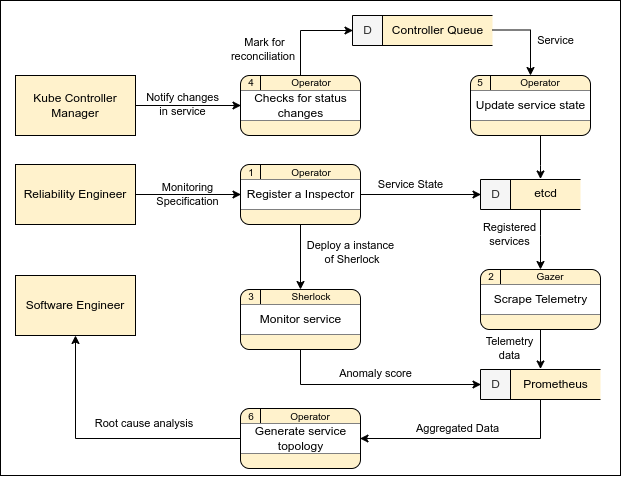
\includegraphics[width=13cm]{assets/system-design/data-flow-level-1.png}
    \caption{Data-flow diagram - level 1 (self-composed)}
    % \label{fig:data-flow}
\end{figure}

\begin{figure}[H]
    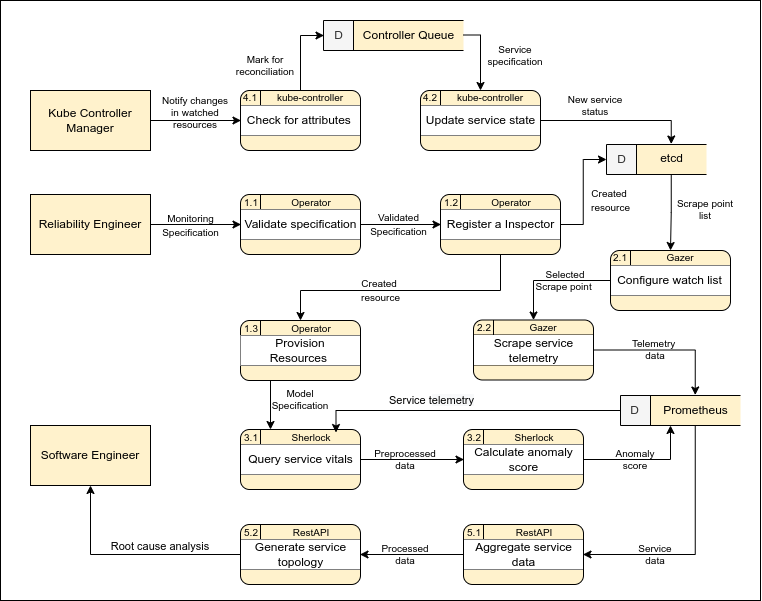
\includegraphics[width=15cm]{assets/system-design/data-flow-level-2.png}
    \caption{Data-flow diagram - level 2 (self-composed)}
    % \label{fig:data-flow}
\end{figure}


\subsection{Sequence Diagram}

Sequences diagrams are meant to showcase the flow of instructions within sub-components of the system. Digrams below explains how the system reacts when two of the main core functionality are invoked.

\begin{figure}[H]
    \centering
    \begin{subfigure}[b]{0.70\textwidth}
        \centering
        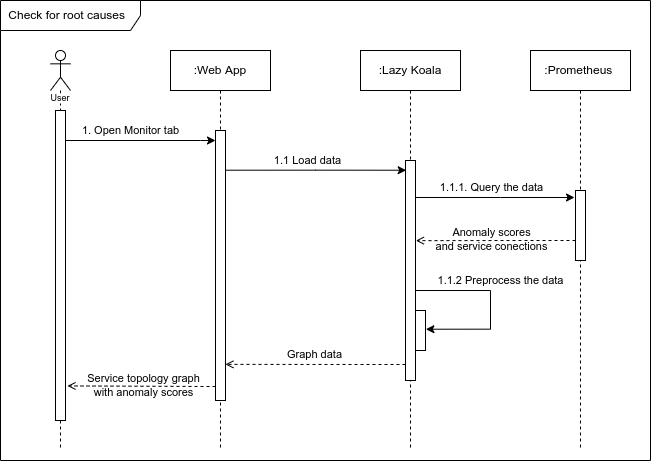
\includegraphics[width=\textwidth]{assets/system-design/sequence-diagram-1.png}
        \caption{Check for root cause}
    \end{subfigure}
    \hfill
    \begin{subfigure}[b]{0.70\textwidth}
        \centering
        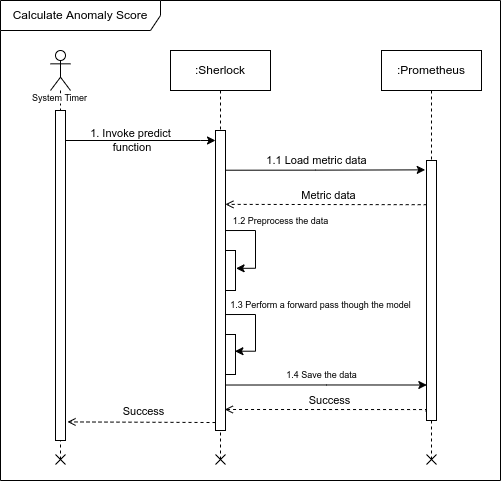
\includegraphics[width=\textwidth]{assets/system-design/sequence-diagram-2.png}
        \caption{Calculate anomaly score}
    \end{subfigure}
    \hfill
       \caption{Sequence diagrams (self-composed)}
\end{figure}

\subsection{UI Design}

Since this project was developed as a Kubernetes native application most of the functionality work as a daemon process in the background. However, there are two use cases where having a visual user interface greatly increases the usability of this project. UI mockups attached below showcase two of those use-cases. Figure \ref{fig:ui-home} displays how developers will be able to inspect the topology of the system and find issues in a realtime while, Figure \ref{fig:ui-settings} showcase the settings page which is used to tag interested services in the system which needs to be monitored.

\begin{figure}[H]
    \centering
    \begin{subfigure}[b]{0.75\textwidth}
        \centering
        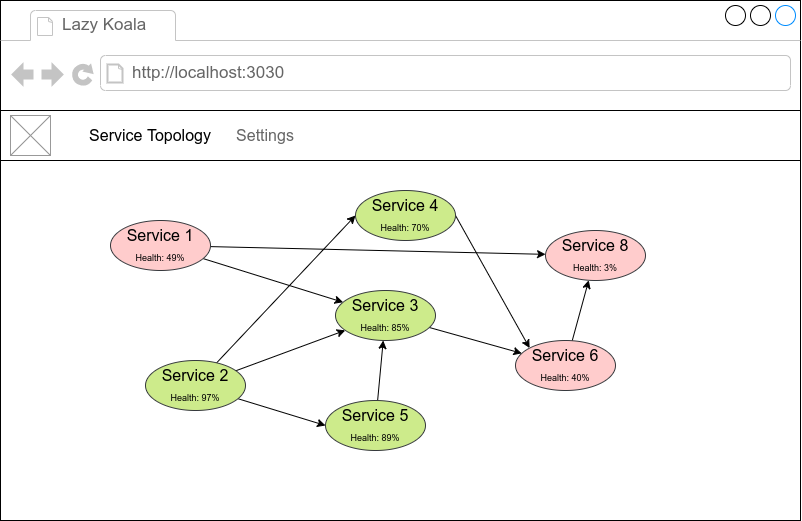
\includegraphics[width=\textwidth]{assets/system-design/ui-home.png}
        \caption{Inspector View}
        \label{fig:ui-home}
    \end{subfigure}
    \hfill
    \begin{subfigure}[b]{0.75\textwidth}
        \centering
        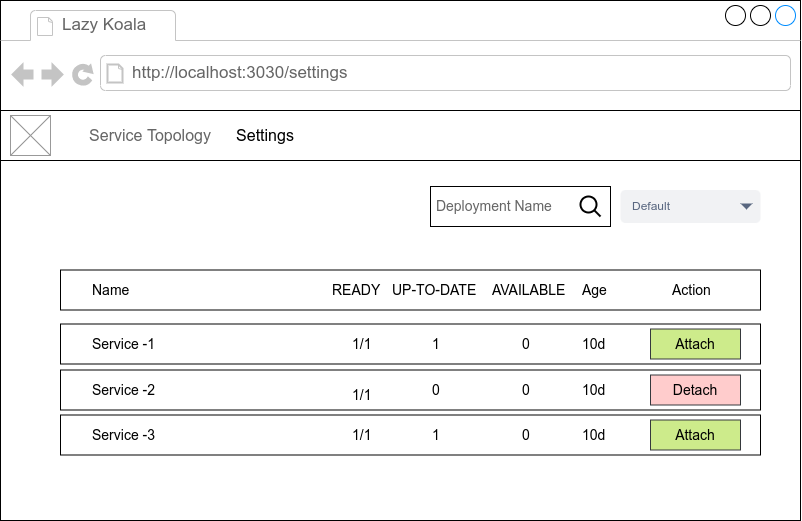
\includegraphics[width=\textwidth]{assets/system-design/ui-settings.png}
        \caption{Settings View}
        \label{fig:ui-settings}
    \end{subfigure}
    \hfill
    % \label{fig:ui-mocks}
    \caption{UI mockups (self-composed)}
\end{figure}